\documentclass[1p]{elsarticle_modified}
%\bibliographystyle{elsarticle-num}

%\usepackage[colorlinks]{hyperref}
%\usepackage{abbrmath_seonhwa} %\Abb, \Ascr, \Acal ,\Abf, \Afrak
\usepackage{amsfonts}
\usepackage{amssymb}
\usepackage{amsmath}
\usepackage{amsthm}
\usepackage{scalefnt}
\usepackage{amsbsy}
\usepackage{kotex}
\usepackage{caption}
\usepackage{subfig}
\usepackage{color}
\usepackage{graphicx}
\usepackage{xcolor} %% white, black, red, green, blue, cyan, magenta, yellow
\usepackage{float}
\usepackage{setspace}
\usepackage{hyperref}

\usepackage{tikz}
\usetikzlibrary{arrows}

\usepackage{multirow}
\usepackage{array} % fixed length table
\usepackage{hhline}

%%%%%%%%%%%%%%%%%%%%%
\makeatletter
\renewcommand*\env@matrix[1][\arraystretch]{%
	\edef\arraystretch{#1}%
	\hskip -\arraycolsep
	\let\@ifnextchar\new@ifnextchar
	\array{*\c@MaxMatrixCols c}}
\makeatother %https://tex.stackexchange.com/questions/14071/how-can-i-increase-the-line-spacing-in-a-matrix
%%%%%%%%%%%%%%%

\usepackage[normalem]{ulem}

\newcommand{\msout}[1]{\ifmmode\text{\sout{\ensuremath{#1}}}\else\sout{#1}\fi}
%SOURCE: \msout is \stkout macro in https://tex.stackexchange.com/questions/20609/strikeout-in-math-mode

\newcommand{\cancel}[1]{
	\ifmmode
	{\color{red}\msout{#1}}
	\else
	{\color{red}\sout{#1}}
	\fi
}

\newcommand{\add}[1]{
	{\color{blue}\uwave{#1}}
}

\newcommand{\replace}[2]{
	\ifmmode
	{\color{red}\msout{#1}}{\color{blue}\uwave{#2}}
	\else
	{\color{red}\sout{#1}}{\color{blue}\uwave{#2}}
	\fi
}

\newcommand{\Sol}{\mathcal{S}} %segment
\newcommand{\D}{D} %diagram
\newcommand{\A}{\mathcal{A}} %arc


%%%%%%%%%%%%%%%%%%%%%%%%%%%%%5 test

\def\sl{\operatorname{\textup{SL}}(2,\Cbb)}
\def\psl{\operatorname{\textup{PSL}}(2,\Cbb)}
\def\quan{\mkern 1mu \triangleright \mkern 1mu}

\theoremstyle{definition}
\newtheorem{thm}{Theorem}[section]
\newtheorem{prop}[thm]{Proposition}
\newtheorem{lem}[thm]{Lemma}
\newtheorem{ques}[thm]{Question}
\newtheorem{cor}[thm]{Corollary}
\newtheorem{defn}[thm]{Definition}
\newtheorem{exam}[thm]{Example}
\newtheorem{rmk}[thm]{Remark}
\newtheorem{alg}[thm]{Algorithm}

\newcommand{\I}{\sqrt{-1}}
\begin{document}

%\begin{frontmatter}
%
%\title{Boundary parabolic representations of knots up to 8 crossings}
%
%%% Group authors per affiliation:
%\author{Yunhi Cho} 
%\address{Department of Mathematics, University of Seoul, Seoul, Korea}
%\ead{yhcho@uos.ac.kr}
%
%
%\author{Seonhwa Kim} %\fnref{s_kim}}
%\address{Center for Geometry and Physics, Institute for Basic Science, Pohang, 37673, Korea}
%\ead{ryeona17@ibs.re.kr}
%
%\author{Hyuk Kim}
%\address{Department of Mathematical Sciences, Seoul National University, Seoul 08826, Korea}
%\ead{hyukkim@snu.ac.kr}
%
%\author{Seokbeom Yoon}
%\address{Department of Mathematical Sciences, Seoul National University, Seoul, 08826,  Korea}
%\ead{sbyoon15@snu.ac.kr}
%
%\begin{abstract}
%We find all boundary parabolic representation of knots up to 8 crossings.
%
%\end{abstract}
%\begin{keyword}
%    \MSC[2010] 57M25 
%\end{keyword}
%
%\end{frontmatter}

%\linenumbers
%\tableofcontents
%
\newcommand\colored[1]{\textcolor{white}{\rule[-0.35ex]{0.8em}{1.4ex}}\kern-0.8em\color{red} #1}%
%\newcommand\colored[1]{\textcolor{white}{ #1}\kern-2.17ex	\textcolor{white}{ #1}\kern-1.81ex	\textcolor{white}{ #1}\kern-2.15ex\color{red}#1	}

{\Large $\underline{12a_{0694}~(K12a_{0694})}$}

\setlength{\tabcolsep}{10pt}
\renewcommand{\arraystretch}{1.6}
\vspace{1cm}\begin{tabular}{m{100pt}>{\centering\arraybackslash}m{274pt}}
\multirow{5}{120pt}{
	\centering
	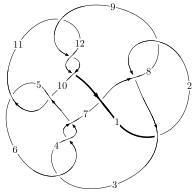
\includegraphics[width=112pt]{../../../GIT/diagram.site/Diagrams/png/1495_12a_0694.png}\\
\ \ \ A knot diagram\footnotemark}&
\allowdisplaybreaks
\textbf{Linearized knot diagam} \\
\cline{2-2}
 &
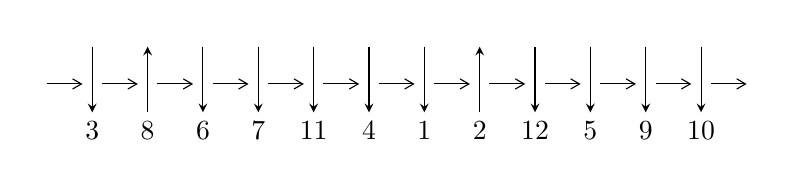
\begin{tikzpicture}[x=20pt, y=17pt]
	% nodes
	\node (C0) at (0, 0) {};
	\node (C1) at (1, 0) {};
	\node (C1U) at (1, +1) {};
	\node (C1D) at (1, -1) {3};

	\node (C2) at (2, 0) {};
	\node (C2U) at (2, +1) {};
	\node (C2D) at (2, -1) {8};

	\node (C3) at (3, 0) {};
	\node (C3U) at (3, +1) {};
	\node (C3D) at (3, -1) {6};

	\node (C4) at (4, 0) {};
	\node (C4U) at (4, +1) {};
	\node (C4D) at (4, -1) {7};

	\node (C5) at (5, 0) {};
	\node (C5U) at (5, +1) {};
	\node (C5D) at (5, -1) {11};

	\node (C6) at (6, 0) {};
	\node (C6U) at (6, +1) {};
	\node (C6D) at (6, -1) {4};

	\node (C7) at (7, 0) {};
	\node (C7U) at (7, +1) {};
	\node (C7D) at (7, -1) {1};

	\node (C8) at (8, 0) {};
	\node (C8U) at (8, +1) {};
	\node (C8D) at (8, -1) {2};

	\node (C9) at (9, 0) {};
	\node (C9U) at (9, +1) {};
	\node (C9D) at (9, -1) {12};

	\node (C10) at (10, 0) {};
	\node (C10U) at (10, +1) {};
	\node (C10D) at (10, -1) {5};

	\node (C11) at (11, 0) {};
	\node (C11U) at (11, +1) {};
	\node (C11D) at (11, -1) {9};

	\node (C12) at (12, 0) {};
	\node (C12U) at (12, +1) {};
	\node (C12D) at (12, -1) {10};
	\node (C13) at (13, 0) {};

	% arrows
	\draw[->,>={angle 60}]
	(C0) edge (C1) (C1) edge (C2) (C2) edge (C3) (C3) edge (C4) (C4) edge (C5) (C5) edge (C6) (C6) edge (C7) (C7) edge (C8) (C8) edge (C9) (C9) edge (C10) (C10) edge (C11) (C11) edge (C12) (C12) edge (C13) ;	\draw[->,>=stealth]
	(C1U) edge (C1D) (C2D) edge (C2U) (C3U) edge (C3D) (C4U) edge (C4D) (C5U) edge (C5D) (C6U) edge (C6D) (C7U) edge (C7D) (C8D) edge (C8U) (C9U) edge (C9D) (C10U) edge (C10D) (C11U) edge (C11D) (C12U) edge (C12D) ;
	\end{tikzpicture} \\
\hhline{~~} \\& 
\textbf{Solving Sequence} \\ \cline{2-2} 
 &
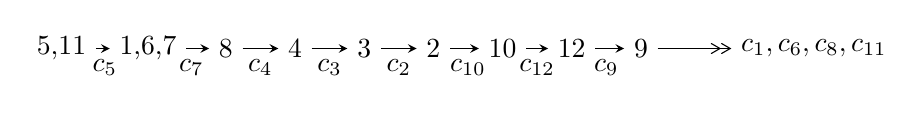
\begin{tikzpicture}[x=25pt, y=7pt]
	% node
	\node (A0) at (-1/8, 0) {5,11};
	\node (A1) at (9/8, 0) {1,6,7};
	\node (A2) at (9/4, 0) {8};
	\node (A3) at (13/4, 0) {4};
	\node (A4) at (17/4, 0) {3};
	\node (A5) at (21/4, 0) {2};
	\node (A6) at (25/4, 0) {10};
	\node (A7) at (29/4, 0) {12};
	\node (A8) at (33/4, 0) {9};
	\node (C1) at (1/2, -1) {$c_{5}$};
	\node (C2) at (7/4, -1) {$c_{7}$};
	\node (C3) at (11/4, -1) {$c_{4}$};
	\node (C4) at (15/4, -1) {$c_{3}$};
	\node (C5) at (19/4, -1) {$c_{2}$};
	\node (C6) at (23/4, -1) {$c_{10}$};
	\node (C7) at (27/4, -1) {$c_{12}$};
	\node (C8) at (31/4, -1) {$c_{9}$};
	\node (A9) at (43/4, 0) {$c_{1},c_{6},c_{8},c_{11}$};

	% edge
	\draw[->,>=stealth]	
	(A0) edge (A1) (A1) edge (A2) (A2) edge (A3) (A3) edge (A4) (A4) edge (A5) (A5) edge (A6) (A6) edge (A7) (A7) edge (A8) ;
	\draw[->>,>={angle 60}]	
	(A8) edge (A9);
\end{tikzpicture} \\ 

\end{tabular} \\

\footnotetext{
The image of knot diagram is generated by the software ``\textbf{Draw programme}" developed by Andrew Bartholomew(\url{http://www.layer8.co.uk/maths/draw/index.htm\#Running-draw}), where we modified some parts for our purpose(\url{https://github.com/CATsTAILs/LinksPainter}).
}\phantom \\ \newline 
\centering \textbf{Ideals for irreducible components\footnotemark of $X_{\text{par}}$} 
 
\begin{align*}
I^u_{1}&=\langle 
3.71327\times10^{48} u^{35}+4.04621\times10^{50} u^{34}+\cdots+1.08619\times10^{53} d-2.28969\times10^{52},\\
\phantom{I^u_{1}}&\phantom{= \langle  }-5.18177\times10^{49} u^{35}-5.63360\times10^{50} u^{34}+\cdots+2.17237\times10^{53} c-2.07122\times10^{53},\\
\phantom{I^u_{1}}&\phantom{= \langle  }-5.97435\times10^{50} u^{35}-1.74229\times10^{51} u^{34}+\cdots+1.08619\times10^{53} b+9.47908\times10^{50},\\
\phantom{I^u_{1}}&\phantom{= \langle  }-2.62593\times10^{51} u^{35}-7.78518\times10^{51} u^{34}+\cdots+2.17237\times10^{53} a+6.90156\times10^{51},\\
\phantom{I^u_{1}}&\phantom{= \langle  }u^{36}+3 u^{35}+\cdots+64 u+32\rangle \\
I^u_{2}&=\langle 
302671644024258 u^{27} a+662808669960639 u^{27}+\cdots-2916745959458060 a-4296331597385486,\\
\phantom{I^u_{2}}&\phantom{= \langle  }5.46608\times10^{15} a u^{27}+5.56735\times10^{15} u^{27}+\cdots-2.36686\times10^{16} a-1.71489\times10^{15},\\
\phantom{I^u_{2}}&\phantom{= \langle  }-7.29186\times10^{14} a u^{27}-8.99105\times10^{14} u^{27}+\cdots+4.25539\times10^{15} a+3.18374\times10^{15},\\
\phantom{I^u_{2}}&\phantom{= \langle  }4247989817783 u^{27} a-203084799592924 u^{27}+\cdots+250742454402200 a+1119525361661648,\\
\phantom{I^u_{2}}&\phantom{= \langle  }u^{28}- u^{27}+\cdots-8 u+4\rangle \\
\\
I^v_{1}&=\langle 
a,\;d,\;c-1,\;b+v+1,\;v^2+v+1\rangle \\
I^v_{2}&=\langle 
c,\;d-1,\;b,\;a- v,\;v^2+v+1\rangle \\
I^v_{3}&=\langle 
a,\;d-1,\;c+a,\;b+1,\;v+1\rangle \\
I^v_{4}&=\langle 
c,\;d-1,\;a^2 v^2-2 c a v+v^2 a+c^2- c v+v^2,\;b v-1\rangle \\
\end{align*}
\raggedright * 5 irreducible components of $\dim_{\mathbb{C}}=0$, with total 97 representations.\\
\raggedright * 1 irreducible components of $\dim_{\mathbb{C}}=1$ \\
\footnotetext{All coefficients of polynomials are rational numbers. But the coefficients are sometimes approximated in decimal forms when there is not enough margin.}
\newpage
\renewcommand{\arraystretch}{1}
\centering \section*{I. $I^u_{1}= \langle 3.71\times10^{48} u^{35}+4.05\times10^{50} u^{34}+\cdots+1.09\times10^{53} d-2.29\times10^{52},\;-5.18\times10^{49} u^{35}-5.63\times10^{50} u^{34}+\cdots+2.17\times10^{53} c-2.07\times10^{53},\;-5.97\times10^{50} u^{35}-1.74\times10^{51} u^{34}+\cdots+1.09\times10^{53} b+9.48\times10^{50},\;-2.63\times10^{51} u^{35}-7.79\times10^{51} u^{34}+\cdots+2.17\times10^{53} a+6.90\times10^{51},\;u^{36}+3 u^{35}+\cdots+64 u+32 \rangle$}
\flushleft \textbf{(i) Arc colorings}\\
\begin{tabular}{m{7pt} m{180pt} m{7pt} m{180pt} }
\flushright $a_{5}=$&$\begin{pmatrix}1\\0\end{pmatrix}$ \\
\flushright $a_{11}=$&$\begin{pmatrix}0\\u\end{pmatrix}$ \\
\flushright $a_{1}=$&$\begin{pmatrix}0.0120878 u^{35}+0.0358372 u^{34}+\cdots-0.808374 u-0.0317697\\0.00550031 u^{35}+0.0160404 u^{34}+\cdots+0.725183 u-0.00872695\end{pmatrix}$ \\
\flushright $a_{6}=$&$\begin{pmatrix}1\\u^2\end{pmatrix}$ \\
\flushright $a_{7}=$&$\begin{pmatrix}0.000238531 u^{35}+0.00259330 u^{34}+\cdots-0.119290 u+0.953438\\-0.0000341864 u^{35}-0.00372516 u^{34}+\cdots+0.444645 u+0.210801\end{pmatrix}$ \\
\flushright $a_{8}=$&$\begin{pmatrix}0.00157086 u^{35}+0.0135938 u^{34}+\cdots-1.44591 u+0.372386\\0.00128903 u^{35}-0.00127210 u^{34}+\cdots+0.00984404 u+0.00259441\end{pmatrix}$ \\
\flushright $a_{4}=$&$\begin{pmatrix}0.000238531 u^{35}+0.00259330 u^{34}+\cdots-0.119290 u+0.953438\\-0.000492763 u^{35}+0.00362002 u^{34}+\cdots-0.572452 u-0.270888\end{pmatrix}$ \\
\flushright $a_{3}=$&$\begin{pmatrix}0.000272717 u^{35}+0.00631846 u^{34}+\cdots-0.563935 u+0.742637\\-0.000426302 u^{35}+0.00445645 u^{34}+\cdots-0.805392 u-0.386811\end{pmatrix}$ \\
\flushright $a_{2}=$&$\begin{pmatrix}0.00896229 u^{35}+0.0251058 u^{34}+\cdots-2.42424 u-0.0549226\\0.0194270 u^{35}+0.0554189 u^{34}+\cdots+0.0990461 u+0.00672681\end{pmatrix}$ \\
\flushright $a_{10}=$&$\begin{pmatrix}u\\u\end{pmatrix}$ \\
\flushright $a_{12}=$&$\begin{pmatrix}0.00846525 u^{35}+0.0249030 u^{34}+\cdots-0.595385 u-0.0306758\\0.00187771 u^{35}+0.00510617 u^{34}+\cdots+0.938172 u-0.00763298\end{pmatrix}$ \\
\flushright $a_{9}=$&$\begin{pmatrix}-0.00658754 u^{35}-0.0197968 u^{34}+\cdots+1.53356 u+0.0230428\\0.00187771 u^{35}+0.00510617 u^{34}+\cdots+0.938172 u-0.00763298\end{pmatrix}$\\&\end{tabular}
\flushleft \textbf{(ii) Obstruction class $= -1$}\\~\\
\flushleft \textbf{(iii) Cusp Shapes $= -0.0805025 u^{35}-0.242112 u^{34}+\cdots-5.72407 u-9.52193$}\\~\\
\newpage\renewcommand{\arraystretch}{1}
\flushleft \textbf{(iv) u-Polynomials at the component}\newline \\
\begin{tabular}{m{50pt}|m{274pt}}
Crossings & \hspace{64pt}u-Polynomials at each crossing \\
\hline $$\begin{aligned}c_{1}\end{aligned}$$&$\begin{aligned}
&u^{36}+17 u^{35}+\cdots-120 u+16
\end{aligned}$\\
\hline $$\begin{aligned}c_{2},c_{8}\end{aligned}$$&$\begin{aligned}
&u^{36}+u^{35}+\cdots+16 u+4
\end{aligned}$\\
\hline $$\begin{aligned}c_{3},c_{4},c_{6}\\c_{9},c_{11},c_{12}\end{aligned}$$&$\begin{aligned}
&u^{36}-5 u^{35}+\cdots+3 u-1
\end{aligned}$\\
\hline $$\begin{aligned}c_{5},c_{10}\end{aligned}$$&$\begin{aligned}
&u^{36}+3 u^{35}+\cdots+64 u+32
\end{aligned}$\\
\hline $$\begin{aligned}c_{7}\end{aligned}$$&$\begin{aligned}
&u^{36}- u^{35}+\cdots-104 u+1252
\end{aligned}$\\
\hline
\end{tabular}\\~\\
\newpage\renewcommand{\arraystretch}{1}
\flushleft \textbf{(v) Riley Polynomials at the component}\newline \\
\begin{tabular}{m{50pt}|m{274pt}}
Crossings & \hspace{64pt}Riley Polynomials at each crossing \\
\hline $$\begin{aligned}c_{1}\end{aligned}$$&$\begin{aligned}
&y^{36}+5 y^{35}+\cdots-27936 y+256
\end{aligned}$\\
\hline $$\begin{aligned}c_{2},c_{8}\end{aligned}$$&$\begin{aligned}
&y^{36}+17 y^{35}+\cdots-120 y+16
\end{aligned}$\\
\hline $$\begin{aligned}c_{3},c_{4},c_{6}\\c_{9},c_{11},c_{12}\end{aligned}$$&$\begin{aligned}
&y^{36}-41 y^{35}+\cdots-21 y+1
\end{aligned}$\\
\hline $$\begin{aligned}c_{5},c_{10}\end{aligned}$$&$\begin{aligned}
&y^{36}-15 y^{35}+\cdots-1024 y+1024
\end{aligned}$\\
\hline $$\begin{aligned}c_{7}\end{aligned}$$&$\begin{aligned}
&y^{36}-7 y^{35}+\cdots-22103608 y+1567504
\end{aligned}$\\
\hline
\end{tabular}\\~\\
\newpage\flushleft \textbf{(vi) Complex Volumes and Cusp Shapes}
$$\begin{array}{c|c|c}  
\text{Solutions to }I^u_{1}& \I (\text{vol} + \sqrt{-1}CS) & \text{Cusp shape}\\
 \hline 
\begin{aligned}
u &= -0.956534 + 0.246505 I \\
a &= \phantom{-}0.245175 - 1.269220 I \\
b &= -0.346134 - 0.784654 I \\
c &= \phantom{-}0.587254 + 0.247408 I \\
d &= \phantom{-}0.446161 - 0.609262 I\end{aligned}
 & -2.56616 + 0.65266 I & -13.12638 - 3.31133 I \\ \hline\begin{aligned}
u &= -0.956534 - 0.246505 I \\
a &= \phantom{-}0.245175 + 1.269220 I \\
b &= -0.346134 + 0.784654 I \\
c &= \phantom{-}0.587254 - 0.247408 I \\
d &= \phantom{-}0.446161 + 0.609262 I\end{aligned}
 & -2.56616 - 0.65266 I & -13.12638 + 3.31133 I \\ \hline\begin{aligned}
u &= \phantom{-}0.935949 + 0.527292 I \\
a &= \phantom{-}0.386487 - 1.298670 I \\
b &= \phantom{-}0.910276 - 0.817885 I \\
c &= \phantom{-}0.601278 - 0.353058 I \\
d &= \phantom{-}0.236726 + 0.726179 I\end{aligned}
 & \phantom{-}1.36964 - 3.10356 I & -5.16268 + 4.71165 I \\ \hline\begin{aligned}
u &= \phantom{-}0.935949 - 0.527292 I \\
a &= \phantom{-}0.386487 + 1.298670 I \\
b &= \phantom{-}0.910276 + 0.817885 I \\
c &= \phantom{-}0.601278 + 0.353058 I \\
d &= \phantom{-}0.236726 - 0.726179 I\end{aligned}
 & \phantom{-}1.36964 + 3.10356 I & -5.16268 - 4.71165 I \\ \hline\begin{aligned}
u &= \phantom{-}0.651308 + 0.620650 I \\
a &= \phantom{-}0.626981 - 0.691158 I \\
b &= \phantom{-}1.099680 - 0.225491 I \\
c &= \phantom{-}0.730839 - 0.428002 I \\
d &= \phantom{-}0.018859 + 0.596676 I\end{aligned}
 & \phantom{-}2.25394 - 1.43184 I & -2.05632 + 3.52848 I \\ \hline\begin{aligned}
u &= \phantom{-}0.651308 - 0.620650 I \\
a &= \phantom{-}0.626981 + 0.691158 I \\
b &= \phantom{-}1.099680 + 0.225491 I \\
c &= \phantom{-}0.730839 + 0.428002 I \\
d &= \phantom{-}0.018859 - 0.596676 I\end{aligned}
 & \phantom{-}2.25394 + 1.43184 I & -2.05632 - 3.52848 I\\
 \hline 
 \end{array}$$\newpage$$\begin{array}{c|c|c}  
\text{Solutions to }I^u_{1}& \I (\text{vol} + \sqrt{-1}CS) & \text{Cusp shape}\\
 \hline 
\begin{aligned}
u &= \phantom{-}0.134519 + 0.831817 I \\
a &= -0.333054 + 0.814839 I \\
b &= -0.168798 - 0.656332 I \\
c &= \phantom{-}0.444936 + 0.012138 I \\
d &= \phantom{-}1.245840 - 0.061269 I\end{aligned}
 & -4.07214 + 2.53804 I & -12.12047 - 3.16226 I \\ \hline\begin{aligned}
u &= \phantom{-}0.134519 - 0.831817 I \\
a &= -0.333054 - 0.814839 I \\
b &= -0.168798 + 0.656332 I \\
c &= \phantom{-}0.444936 - 0.012138 I \\
d &= \phantom{-}1.245840 + 0.061269 I\end{aligned}
 & -4.07214 - 2.53804 I & -12.12047 + 3.16226 I \\ \hline\begin{aligned}
u &= -0.488093 + 0.675929 I \\
a &= -0.729751 - 0.351432 I \\
b &= -1.163350 + 0.137978 I \\
c &= \phantom{-}0.831879 + 0.502397 I \\
d &= -0.119169 - 0.531960 I\end{aligned}
 & \phantom{-}0.92725 - 3.15352 I & -4.07893 + 3.45921 I \\ \hline\begin{aligned}
u &= -0.488093 - 0.675929 I \\
a &= -0.729751 + 0.351432 I \\
b &= -1.163350 - 0.137978 I \\
c &= \phantom{-}0.831879 - 0.502397 I \\
d &= -0.119169 + 0.531960 I\end{aligned}
 & \phantom{-}0.92725 + 3.15352 I & -4.07893 - 3.45921 I \\ \hline\begin{aligned}
u &= -1.066500 + 0.529753 I \\
a &= -0.36138 - 1.59734 I \\
b &= -0.887704 - 1.098310 I \\
c &= \phantom{-}0.554284 + 0.346614 I \\
d &= \phantom{-}0.296959 - 0.811036 I\end{aligned}
 & -0.85359 + 7.85577 I & -9.34096 - 8.43490 I \\ \hline\begin{aligned}
u &= -1.066500 - 0.529753 I \\
a &= -0.36138 + 1.59734 I \\
b &= -0.887704 + 1.098310 I \\
c &= \phantom{-}0.554284 - 0.346614 I \\
d &= \phantom{-}0.296959 + 0.811036 I\end{aligned}
 & -0.85359 - 7.85577 I & -9.34096 + 8.43490 I\\
 \hline 
 \end{array}$$\newpage$$\begin{array}{c|c|c}  
\text{Solutions to }I^u_{1}& \I (\text{vol} + \sqrt{-1}CS) & \text{Cusp shape}\\
 \hline 
\begin{aligned}
u &= \phantom{-}0.471804 + 1.201650 I \\
a &= -1.033650 - 0.000390 I \\
b &= -0.795501 - 1.088210 I \\
c &= \phantom{-}0.409694 + 0.038448 I \\
d &= \phantom{-}1.41953 - 0.22707 I\end{aligned}
 & -6.92260 + 4.39379 I & -12.55418 - 2.40542 I \\ \hline\begin{aligned}
u &= \phantom{-}0.471804 - 1.201650 I \\
a &= -1.033650 + 0.000390 I \\
b &= -0.795501 + 1.088210 I \\
c &= \phantom{-}0.409694 - 0.038448 I \\
d &= \phantom{-}1.41953 + 0.22707 I\end{aligned}
 & -6.92260 - 4.39379 I & -12.55418 + 2.40542 I \\ \hline\begin{aligned}
u &= -1.232210 + 0.408112 I \\
a &= -0.074767 + 0.904861 I \\
b &= \phantom{-}1.02170 + 1.10904 I \\
c &= -1.91298 - 0.86265 I \\
d &= -1.43441 + 0.19589 I\end{aligned}
 & -8.11992 + 1.67660 I & -15.7568 - 0.9806 I \\ \hline\begin{aligned}
u &= -1.232210 - 0.408112 I \\
a &= -0.074767 - 0.904861 I \\
b &= \phantom{-}1.02170 - 1.10904 I \\
c &= -1.91298 + 0.86265 I \\
d &= -1.43441 - 0.19589 I\end{aligned}
 & -8.11992 - 1.67660 I & -15.7568 + 0.9806 I \\ \hline\begin{aligned}
u &= \phantom{-}1.223950 + 0.516090 I \\
a &= \phantom{-}0.037576 + 1.129580 I \\
b &= -1.02760 + 1.37545 I \\
c &= -1.74112 + 1.00593 I \\
d &= -1.43061 - 0.24878 I\end{aligned}
 & -7.33125 - 7.52384 I & -14.0983 + 6.1679 I \\ \hline\begin{aligned}
u &= \phantom{-}1.223950 - 0.516090 I \\
a &= \phantom{-}0.037576 - 1.129580 I \\
b &= -1.02760 - 1.37545 I \\
c &= -1.74112 - 1.00593 I \\
d &= -1.43061 + 0.24878 I\end{aligned}
 & -7.33125 + 7.52384 I & -14.0983 - 6.1679 I\\
 \hline 
 \end{array}$$\newpage$$\begin{array}{c|c|c}  
\text{Solutions to }I^u_{1}& \I (\text{vol} + \sqrt{-1}CS) & \text{Cusp shape}\\
 \hline 
\begin{aligned}
u &= \phantom{-}0.666134 + 0.068993 I \\
a &= -1.123260 + 0.576466 I \\
b &= -0.104353 + 0.169913 I \\
c &= \phantom{-}0.577923 + 0.067898 I \\
d &= \phantom{-}0.706776 - 0.200522 I\end{aligned}
 & -2.77509 + 2.72721 I & -16.6085 - 5.9652 I \\ \hline\begin{aligned}
u &= \phantom{-}0.666134 - 0.068993 I \\
a &= -1.123260 - 0.576466 I \\
b &= -0.104353 - 0.169913 I \\
c &= \phantom{-}0.577923 - 0.067898 I \\
d &= \phantom{-}0.706776 + 0.200522 I\end{aligned}
 & -2.77509 - 2.72721 I & -16.6085 + 5.9652 I \\ \hline\begin{aligned}
u &= -0.318666 + 1.335800 I \\
a &= \phantom{-}0.724523 - 0.313609 I \\
b &= \phantom{-}0.58164 - 1.39075 I \\
c &= \phantom{-}0.401008 - 0.024597 I \\
d &= \phantom{-}1.48437 + 0.15238 I\end{aligned}
 & -11.42670 - 0.95860 I & -17.6650 - 0.2050 I \\ \hline\begin{aligned}
u &= -0.318666 - 1.335800 I \\
a &= \phantom{-}0.724523 + 0.313609 I \\
b &= \phantom{-}0.58164 + 1.39075 I \\
c &= \phantom{-}0.401008 + 0.024597 I \\
d &= \phantom{-}1.48437 - 0.15238 I\end{aligned}
 & -11.42670 + 0.95860 I & -17.6650 + 0.2050 I \\ \hline\begin{aligned}
u &= -0.568640 + 1.285090 I \\
a &= \phantom{-}1.254760 - 0.150682 I \\
b &= \phantom{-}1.01253 - 1.18042 I \\
c &= \phantom{-}0.401346 - 0.044727 I \\
d &= \phantom{-}1.46105 + 0.27427 I\end{aligned}
 & -9.63713 - 9.42250 I & -15.4804 + 5.9490 I \\ \hline\begin{aligned}
u &= -0.568640 - 1.285090 I \\
a &= \phantom{-}1.254760 + 0.150682 I \\
b &= \phantom{-}1.01253 + 1.18042 I \\
c &= \phantom{-}0.401346 + 0.044727 I \\
d &= \phantom{-}1.46105 - 0.27427 I\end{aligned}
 & -9.63713 + 9.42250 I & -15.4804 - 5.9490 I\\
 \hline 
 \end{array}$$\newpage$$\begin{array}{c|c|c}  
\text{Solutions to }I^u_{1}& \I (\text{vol} + \sqrt{-1}CS) & \text{Cusp shape}\\
 \hline 
\begin{aligned}
u &= -0.579877\phantom{ +0.000000I} \\
a &= \phantom{-}0.508844\phantom{ +0.000000I} \\
b &= -0.181813\phantom{ +0.000000I} \\
c &= \phantom{-}0.714033\phantom{ +0.000000I} \\
d &= \phantom{-}0.400496\phantom{ +0.000000I}\end{aligned}
 & -0.811618\phantom{ +0.000000I} & -12.0290\phantom{ +0.000000I} \\ \hline\begin{aligned}
u &= \phantom{-}1.27702 + 0.74720 I \\
a &= \phantom{-}0.06527 + 1.61805 I \\
b &= -0.91000 + 1.90449 I \\
c &= -1.34025 + 1.05868 I \\
d &= -1.45945 - 0.36293 I\end{aligned}
 & -9.5381 - 11.3478 I & -13.0594 + 5.6672 I \\ \hline\begin{aligned}
u &= \phantom{-}1.27702 - 0.74720 I \\
a &= \phantom{-}0.06527 - 1.61805 I \\
b &= -0.91000 - 1.90449 I \\
c &= -1.34025 - 1.05868 I \\
d &= -1.45945 + 0.36293 I\end{aligned}
 & -9.5381 + 11.3478 I & -13.0594 - 5.6672 I \\ \hline\begin{aligned}
u &= -1.51924\phantom{ +0.000000I} \\
a &= -0.762049\phantom{ +0.000000I} \\
b &= \phantom{-}0.272206\phantom{ +0.000000I} \\
c &= -1.75045\phantom{ +0.000000I} \\
d &= -1.57128\phantom{ +0.000000I}\end{aligned}
 & -14.8609\phantom{ +0.000000I} & -15.8600\phantom{ +0.000000I} \\ \hline\begin{aligned}
u &= -1.29117 + 0.81558 I \\
a &= -0.05855 + 1.76313 I \\
b &= \phantom{-}0.89290 + 2.05678 I \\
c &= -1.24306 - 1.05406 I \\
d &= -1.46798 + 0.39682 I\end{aligned}
 & -12.0349 + 16.8809 I & -15.3736 - 9.2575 I \\ \hline\begin{aligned}
u &= -1.29117 - 0.81558 I \\
a &= -0.05855 - 1.76313 I \\
b &= \phantom{-}0.89290 - 2.05678 I \\
c &= -1.24306 + 1.05406 I \\
d &= -1.46798 - 0.39682 I\end{aligned}
 & -12.0349 - 16.8809 I & -15.3736 + 9.2575 I\\
 \hline 
 \end{array}$$\newpage$$\begin{array}{c|c|c}  
\text{Solutions to }I^u_{1}& \I (\text{vol} + \sqrt{-1}CS) & \text{Cusp shape}\\
 \hline 
\begin{aligned}
u &= -0.111921 + 0.451208 I \\
a &= -0.148541 + 0.145650 I \\
b &= -0.283161 + 0.602030 I \\
c &= \phantom{-}1.212710 + 0.167592 I \\
d &= -0.190856 - 0.111820 I\end{aligned}
 & -0.30692 + 1.79670 I & -2.13838 - 3.34715 I \\ \hline\begin{aligned}
u &= -0.111921 - 0.451208 I \\
a &= -0.148541 - 0.145650 I \\
b &= -0.283161 - 0.602030 I \\
c &= \phantom{-}1.212710 - 0.167592 I \\
d &= -0.190856 + 0.111820 I\end{aligned}
 & -0.30692 - 1.79670 I & -2.13838 + 3.34715 I \\ \hline\begin{aligned}
u &= -1.38860 + 0.67758 I \\
a &= -0.32966 + 1.52385 I \\
b &= \phantom{-}0.64328 + 1.76352 I \\
c &= -1.38705 - 0.88191 I \\
d &= -1.51341 + 0.32643 I\end{aligned}
 & -15.0030 + 8.0885 I & -18.3300 - 3.8436 I \\ \hline\begin{aligned}
u &= -1.38860 - 0.67758 I \\
a &= -0.32966 - 1.52385 I \\
b &= \phantom{-}0.64328 - 1.76352 I \\
c &= -1.38705 + 0.88191 I \\
d &= -1.51341 - 0.32643 I\end{aligned}
 & -15.0030 - 8.0885 I & -18.3300 + 3.8436 I \\ \hline\begin{aligned}
u &= \phantom{-}1.61122 + 0.12770 I \\
a &= \phantom{-}0.978439 + 0.310581 I \\
b &= -0.020607 + 0.352320 I \\
c &= -1.61050 + 0.15798 I \\
d &= -1.61501 - 0.06033 I\end{aligned}
 & -18.8051 - 4.7571 I & -19.1049 + 3.2273 I \\ \hline\begin{aligned}
u &= \phantom{-}1.61122 - 0.12770 I \\
a &= \phantom{-}0.978439 - 0.310581 I \\
b &= -0.020607 - 0.352320 I \\
c &= -1.61050 - 0.15798 I \\
d &= -1.61501 + 0.06033 I\end{aligned}
 & -18.8051 + 4.7571 I & -19.1049 - 3.2273 I\\
 \hline 
 \end{array}$$\newpage\newpage\renewcommand{\arraystretch}{1}
\centering \section*{II. $I^u_{2}= \langle 3.03\times10^{14} a u^{27}+6.63\times10^{14} u^{27}+\cdots-2.92\times10^{15} a-4.30\times10^{15},\;5.47\times10^{15} a u^{27}+5.57\times10^{15} u^{27}+\cdots-2.37\times10^{16} a-1.71\times10^{15},\;-7.29\times10^{14} a u^{27}-8.99\times10^{14} u^{27}+\cdots+4.26\times10^{15} a+3.18\times10^{15},\;4.25\times10^{12} a u^{27}-2.03\times10^{14} u^{27}+\cdots+2.51\times10^{14} a+1.12\times10^{15},\;u^{28}- u^{27}+\cdots-8 u+4 \rangle$}
\flushleft \textbf{(i) Arc colorings}\\
\begin{tabular}{m{7pt} m{180pt} m{7pt} m{180pt} }
\flushright $a_{5}=$&$\begin{pmatrix}1\\0\end{pmatrix}$ \\
\flushright $a_{11}=$&$\begin{pmatrix}0\\u\end{pmatrix}$ \\
\flushright $a_{1}=$&$\begin{pmatrix}a\\2.82492 a u^{27}+3.48319 u^{27}+\cdots-16.4857 a-12.3340\end{pmatrix}$ \\
\flushright $a_{6}=$&$\begin{pmatrix}1\\u^2\end{pmatrix}$ \\
\flushright $a_{7}=$&$\begin{pmatrix}-5.29398 a u^{27}-5.39206 u^{27}+\cdots+22.9234 a+1.66090\\-1.17257 a u^{27}-2.56776 u^{27}+\cdots+11.2997 a+16.6443\end{pmatrix}$ \\
\flushright $a_{8}=$&$\begin{pmatrix}-5.46593 a u^{27}-5.39206 u^{27}+\cdots+21.5903 a+1.66090\\-1.60474 a u^{27}-5.47431 u^{27}+\cdots+15.1316 a+36.9788\end{pmatrix}$ \\
\flushright $a_{4}=$&$\begin{pmatrix}-5.29398 a u^{27}-5.39206 u^{27}+\cdots+22.9234 a+1.66090\\-0.210350 a u^{27}-0.338787 u^{27}+\cdots+1.35515 a+3.69028\end{pmatrix}$ \\
\flushright $a_{3}=$&$\begin{pmatrix}-4.12142 a u^{27}-2.82430 u^{27}+\cdots+11.6237 a-14.9834\\-0.0843068 u^{27}+0.0893064 u^{26}+\cdots-1.10305 u+0.0658279\end{pmatrix}$ \\
\flushright $a_{2}=$&$\begin{pmatrix}-0.0154888 a u^{27}-1.33360 u^{27}+\cdots+1.66131 a-4.83197\\4.22120 a u^{27}+4.90685 u^{27}+\cdots-24.1466 a-20.2576\end{pmatrix}$ \\
\flushright $a_{10}=$&$\begin{pmatrix}u\\u\end{pmatrix}$ \\
\flushright $a_{12}=$&$\begin{pmatrix}0.338787 a u^{27}-0.377991 u^{27}+\cdots-3.69028 a-5.87532\\3.16370 a u^{27}+3.10520 u^{27}+\cdots-21.1759 a-18.2093\end{pmatrix}$ \\
\flushright $a_{9}=$&$\begin{pmatrix}2.82492 a u^{27}+3.48319 u^{27}+\cdots-17.4857 a-12.3340\\3.16370 a u^{27}+3.10520 u^{27}+\cdots-21.1759 a-18.2093\end{pmatrix}$\\&\end{tabular}
\flushleft \textbf{(ii) Obstruction class $= -1$}\\~\\
\flushleft \textbf{(iii) Cusp Shapes $= -\frac{37274533074785}{129063433504426} u^{27}+\frac{53621307092165}{129063433504426} u^{26}+\cdots-\frac{660629047616669}{129063433504426} u-\frac{645502044434670}{64531716752213}$}\\~\\
\newpage\renewcommand{\arraystretch}{1}
\flushleft \textbf{(iv) u-Polynomials at the component}\newline \\
\begin{tabular}{m{50pt}|m{274pt}}
Crossings & \hspace{64pt}u-Polynomials at each crossing \\
\hline $$\begin{aligned}c_{1}\end{aligned}$$&$\begin{aligned}
&(u^{28}+14 u^{27}+\cdots+2 u+1)^{2}
\end{aligned}$\\
\hline $$\begin{aligned}c_{2},c_{8}\end{aligned}$$&$\begin{aligned}
&(u^{28}+2 u^{27}+\cdots+2 u+1)^{2}
\end{aligned}$\\
\hline $$\begin{aligned}c_{3},c_{4},c_{6}\\c_{9},c_{11},c_{12}\end{aligned}$$&$\begin{aligned}
&u^{56}-3 u^{55}+\cdots+72 u+16
\end{aligned}$\\
\hline $$\begin{aligned}c_{5},c_{10}\end{aligned}$$&$\begin{aligned}
&(u^{28}- u^{27}+\cdots-8 u+4)^{2}
\end{aligned}$\\
\hline $$\begin{aligned}c_{7}\end{aligned}$$&$\begin{aligned}
&(u^{28}-2 u^{27}+\cdots-22 u+17)^{2}
\end{aligned}$\\
\hline
\end{tabular}\\~\\
\newpage\renewcommand{\arraystretch}{1}
\flushleft \textbf{(v) Riley Polynomials at the component}\newline \\
\begin{tabular}{m{50pt}|m{274pt}}
Crossings & \hspace{64pt}Riley Polynomials at each crossing \\
\hline $$\begin{aligned}c_{1}\end{aligned}$$&$\begin{aligned}
&(y^{28}+2 y^{27}+\cdots+14 y+1)^{2}
\end{aligned}$\\
\hline $$\begin{aligned}c_{2},c_{8}\end{aligned}$$&$\begin{aligned}
&(y^{28}+14 y^{27}+\cdots+2 y+1)^{2}
\end{aligned}$\\
\hline $$\begin{aligned}c_{3},c_{4},c_{6}\\c_{9},c_{11},c_{12}\end{aligned}$$&$\begin{aligned}
&y^{56}-43 y^{55}+\cdots+736 y+256
\end{aligned}$\\
\hline $$\begin{aligned}c_{5},c_{10}\end{aligned}$$&$\begin{aligned}
&(y^{28}-15 y^{27}+\cdots-88 y+16)^{2}
\end{aligned}$\\
\hline $$\begin{aligned}c_{7}\end{aligned}$$&$\begin{aligned}
&(y^{28}-10 y^{27}+\cdots-246 y+289)^{2}
\end{aligned}$\\
\hline
\end{tabular}\\~\\
\newpage\flushleft \textbf{(vi) Complex Volumes and Cusp Shapes}
$$\begin{array}{c|c|c}  
\text{Solutions to }I^u_{2}& \I (\text{vol} + \sqrt{-1}CS) & \text{Cusp shape}\\
 \hline 
\begin{aligned}
u &= -0.910131 + 0.395689 I \\
a &= \phantom{-}0.577913 + 0.875653 I \\
b &= \phantom{-}1.83296 + 1.21612 I \\
c &= \phantom{-}0.614034 + 0.300820 I \\
d &= \phantom{-}0.313357 - 0.643423 I\end{aligned}
 & -1.72215 + 4.24816 I & -10.11355 - 6.97904 I \\ \hline\begin{aligned}
u &= -0.910131 + 0.395689 I \\
a &= -0.099220 - 1.209090 I \\
b &= -0.647282 - 0.740410 I \\
c &= -2.48219 - 1.67345 I \\
d &= -1.276980 + 0.186733 I\end{aligned}
 & -1.72215 + 4.24816 I & -10.11355 - 6.97904 I \\ \hline\begin{aligned}
u &= -0.910131 - 0.395689 I \\
a &= \phantom{-}0.577913 - 0.875653 I \\
b &= \phantom{-}1.83296 - 1.21612 I \\
c &= \phantom{-}0.614034 - 0.300820 I \\
d &= \phantom{-}0.313357 + 0.643423 I\end{aligned}
 & -1.72215 - 4.24816 I & -10.11355 + 6.97904 I \\ \hline\begin{aligned}
u &= -0.910131 - 0.395689 I \\
a &= -0.099220 + 1.209090 I \\
b &= -0.647282 + 0.740410 I \\
c &= -2.48219 + 1.67345 I \\
d &= -1.276980 - 0.186733 I\end{aligned}
 & -1.72215 - 4.24816 I & -10.11355 + 6.97904 I \\ \hline\begin{aligned}
u &= \phantom{-}0.017123 + 0.961380 I \\
a &= \phantom{-}1.23063 + 0.74510 I \\
b &= \phantom{-}1.77384 + 1.41897 I \\
c &= \phantom{-}0.433525 + 0.001501 I \\
d &= \phantom{-}1.306640 - 0.007988 I\end{aligned}
 & -4.61196 - 1.34593 I & -13.91932 + 0.66126 I \\ \hline\begin{aligned}
u &= \phantom{-}0.017123 + 0.961380 I \\
a &= -0.039967 + 0.519614 I \\
b &= -0.024073 - 0.839235 I \\
c &= \phantom{-}0.86981 - 1.28447 I \\
d &= -0.638546 + 0.533764 I\end{aligned}
 & -4.61196 - 1.34593 I & -13.91932 + 0.66126 I\\
 \hline 
 \end{array}$$\newpage$$\begin{array}{c|c|c}  
\text{Solutions to }I^u_{2}& \I (\text{vol} + \sqrt{-1}CS) & \text{Cusp shape}\\
 \hline 
\begin{aligned}
u &= \phantom{-}0.017123 - 0.961380 I \\
a &= \phantom{-}1.23063 - 0.74510 I \\
b &= \phantom{-}1.77384 - 1.41897 I \\
c &= \phantom{-}0.433525 - 0.001501 I \\
d &= \phantom{-}1.306640 + 0.007988 I\end{aligned}
 & -4.61196 + 1.34593 I & -13.91932 - 0.66126 I \\ \hline\begin{aligned}
u &= \phantom{-}0.017123 - 0.961380 I \\
a &= -0.039967 - 0.519614 I \\
b &= -0.024073 + 0.839235 I \\
c &= \phantom{-}0.86981 + 1.28447 I \\
d &= -0.638546 - 0.533764 I\end{aligned}
 & -4.61196 + 1.34593 I & -13.91932 - 0.66126 I \\ \hline\begin{aligned}
u &= \phantom{-}0.907099 + 0.252760 I \\
a &= -0.216978 - 1.161080 I \\
b &= \phantom{-}0.375545 - 0.694496 I \\
c &= \phantom{-}0.507453 + 0.124235 I \\
d &= \phantom{-}0.859190 - 0.455166 I\end{aligned}
 & -2.63794 - 3.28147 I & -13.2327 + 4.9939 I \\ \hline\begin{aligned}
u &= \phantom{-}0.907099 + 0.252760 I \\
a &= -1.21470 + 1.14721 I \\
b &= -0.465509 + 0.436668 I \\
c &= \phantom{-}0.605754 - 0.244512 I \\
d &= \phantom{-}0.419544 + 0.572998 I\end{aligned}
 & -2.63794 - 3.28147 I & -13.2327 + 4.9939 I \\ \hline\begin{aligned}
u &= \phantom{-}0.907099 - 0.252760 I \\
a &= -0.216978 + 1.161080 I \\
b &= \phantom{-}0.375545 + 0.694496 I \\
c &= \phantom{-}0.507453 - 0.124235 I \\
d &= \phantom{-}0.859190 + 0.455166 I\end{aligned}
 & -2.63794 + 3.28147 I & -13.2327 - 4.9939 I \\ \hline\begin{aligned}
u &= \phantom{-}0.907099 - 0.252760 I \\
a &= -1.21470 - 1.14721 I \\
b &= -0.465509 - 0.436668 I \\
c &= \phantom{-}0.605754 + 0.244512 I \\
d &= \phantom{-}0.419544 - 0.572998 I\end{aligned}
 & -2.63794 + 3.28147 I & -13.2327 - 4.9939 I\\
 \hline 
 \end{array}$$\newpage$$\begin{array}{c|c|c}  
\text{Solutions to }I^u_{2}& \I (\text{vol} + \sqrt{-1}CS) & \text{Cusp shape}\\
 \hline 
\begin{aligned}
u &= -0.387411 + 0.832689 I \\
a &= -1.036680 - 0.102202 I \\
b &= -1.48423 + 0.44182 I \\
c &= \phantom{-}0.443674 - 0.035750 I \\
d &= \phantom{-}1.239370 + 0.180444 I\end{aligned}
 & -1.43770 - 1.40144 I & -7.30053 + 1.74630 I \\ \hline\begin{aligned}
u &= -0.387411 + 0.832689 I \\
a &= \phantom{-}0.879401 + 0.727615 I \\
b &= \phantom{-}0.488283 - 0.578810 I \\
c &= \phantom{-}0.838293 + 0.678920 I \\
d &= -0.279611 - 0.583432 I\end{aligned}
 & -1.43770 - 1.40144 I & -7.30053 + 1.74630 I \\ \hline\begin{aligned}
u &= -0.387411 - 0.832689 I \\
a &= -1.036680 + 0.102202 I \\
b &= -1.48423 - 0.44182 I \\
c &= \phantom{-}0.443674 + 0.035750 I \\
d &= \phantom{-}1.239370 - 0.180444 I\end{aligned}
 & -1.43770 + 1.40144 I & -7.30053 - 1.74630 I \\ \hline\begin{aligned}
u &= -0.387411 - 0.832689 I \\
a &= \phantom{-}0.879401 - 0.727615 I \\
b &= \phantom{-}0.488283 + 0.578810 I \\
c &= \phantom{-}0.838293 - 0.678920 I \\
d &= -0.279611 + 0.583432 I\end{aligned}
 & -1.43770 + 1.40144 I & -7.30053 - 1.74630 I \\ \hline\begin{aligned}
u &= \phantom{-}0.387502 + 1.047530 I \\
a &= -0.847760 + 0.306836 I \\
b &= -0.585544 - 0.879512 I \\
c &= \phantom{-}0.669242 - 0.797085 I \\
d &= -0.382179 + 0.735842 I\end{aligned}
 & -3.70255 + 5.75423 I & -11.89302 - 5.96655 I \\ \hline\begin{aligned}
u &= \phantom{-}0.387502 + 1.047530 I \\
a &= \phantom{-}1.51403 - 0.04211 I \\
b &= \phantom{-}2.01322 + 0.50738 I \\
c &= \phantom{-}0.423917 + 0.033459 I \\
d &= \phantom{-}1.344350 - 0.185032 I\end{aligned}
 & -3.70255 + 5.75423 I & -11.89302 - 5.96655 I\\
 \hline 
 \end{array}$$\newpage$$\begin{array}{c|c|c}  
\text{Solutions to }I^u_{2}& \I (\text{vol} + \sqrt{-1}CS) & \text{Cusp shape}\\
 \hline 
\begin{aligned}
u &= \phantom{-}0.387502 - 1.047530 I \\
a &= -0.847760 - 0.306836 I \\
b &= -0.585544 + 0.879512 I \\
c &= \phantom{-}0.669242 + 0.797085 I \\
d &= -0.382179 - 0.735842 I\end{aligned}
 & -3.70255 - 5.75423 I & -11.89302 + 5.96655 I \\ \hline\begin{aligned}
u &= \phantom{-}0.387502 - 1.047530 I \\
a &= \phantom{-}1.51403 + 0.04211 I \\
b &= \phantom{-}2.01322 - 0.50738 I \\
c &= \phantom{-}0.423917 - 0.033459 I \\
d &= \phantom{-}1.344350 + 0.185032 I\end{aligned}
 & -3.70255 - 5.75423 I & -11.89302 + 5.96655 I \\ \hline\begin{aligned}
u &= \phantom{-}0.802767 + 0.244916 I \\
a &= -0.844969 + 0.599643 I \\
b &= -2.28532 + 0.90013 I \\
c &= \phantom{-}0.647474 - 0.227775 I \\
d &= \phantom{-}0.374376 + 0.483492 I\end{aligned}
 & -2.32218 + 0.90628 I & -12.59768 + 1.67094 I \\ \hline\begin{aligned}
u &= \phantom{-}0.802767 + 0.244916 I \\
a &= -0.201313 - 0.924926 I \\
b &= \phantom{-}0.393435 - 0.504095 I \\
c &= -3.52128 + 1.70882 I \\
d &= -1.229860 - 0.111546 I\end{aligned}
 & -2.32218 + 0.90628 I & -12.59768 + 1.67094 I \\ \hline\begin{aligned}
u &= \phantom{-}0.802767 - 0.244916 I \\
a &= -0.844969 - 0.599643 I \\
b &= -2.28532 - 0.90013 I \\
c &= \phantom{-}0.647474 + 0.227775 I \\
d &= \phantom{-}0.374376 - 0.483492 I\end{aligned}
 & -2.32218 - 0.90628 I & -12.59768 - 1.67094 I \\ \hline\begin{aligned}
u &= \phantom{-}0.802767 - 0.244916 I \\
a &= -0.201313 + 0.924926 I \\
b &= \phantom{-}0.393435 + 0.504095 I \\
c &= -3.52128 - 1.70882 I \\
d &= -1.229860 + 0.111546 I\end{aligned}
 & -2.32218 - 0.90628 I & -12.59768 - 1.67094 I\\
 \hline 
 \end{array}$$\newpage$$\begin{array}{c|c|c}  
\text{Solutions to }I^u_{2}& \I (\text{vol} + \sqrt{-1}CS) & \text{Cusp shape}\\
 \hline 
\begin{aligned}
u &= \phantom{-}1.147340 + 0.340892 I \\
a &= -0.098527 + 0.753717 I \\
b &= -1.25317 + 0.95465 I \\
c &= \phantom{-}0.467659 + 0.149971 I \\
d &= \phantom{-}0.938913 - 0.621780 I\end{aligned}
 & -5.81300 - 1.47542 I & -13.29345 + 0.59666 I \\ \hline\begin{aligned}
u &= \phantom{-}1.147340 + 0.340892 I \\
a &= -1.40778 + 1.44620 I \\
b &= -0.803773 + 0.724816 I \\
c &= -2.16974 + 0.89969 I \\
d &= -1.393270 - 0.163069 I\end{aligned}
 & -5.81300 - 1.47542 I & -13.29345 + 0.59666 I \\ \hline\begin{aligned}
u &= \phantom{-}1.147340 - 0.340892 I \\
a &= -0.098527 - 0.753717 I \\
b &= -1.25317 - 0.95465 I \\
c &= \phantom{-}0.467659 - 0.149971 I \\
d &= \phantom{-}0.938913 + 0.621780 I\end{aligned}
 & -5.81300 + 1.47542 I & -13.29345 - 0.59666 I \\ \hline\begin{aligned}
u &= \phantom{-}1.147340 - 0.340892 I \\
a &= -1.40778 - 1.44620 I \\
b &= -0.803773 - 0.724816 I \\
c &= -2.16974 - 0.89969 I \\
d &= -1.393270 + 0.163069 I\end{aligned}
 & -5.81300 + 1.47542 I & -13.29345 - 0.59666 I \\ \hline\begin{aligned}
u &= -0.611767 + 0.458091 I \\
a &= -0.302684 - 0.597006 I \\
b &= -0.775693 - 0.182328 I \\
c &= \phantom{-}0.484849 - 0.064041 I \\
d &= \phantom{-}1.027130 + 0.267751 I\end{aligned}
 & -0.887541 - 0.644142 I & -7.64602 - 1.30683 I \\ \hline\begin{aligned}
u &= -0.611767 + 0.458091 I \\
a &= \phantom{-}1.34953 + 1.04053 I \\
b &= \phantom{-}0.483743 - 0.045437 I \\
c &= \phantom{-}0.768846 + 0.328940 I \\
d &= \phantom{-}0.099411 - 0.470368 I\end{aligned}
 & -0.887541 - 0.644142 I & -7.64602 - 1.30683 I\\
 \hline 
 \end{array}$$\newpage$$\begin{array}{c|c|c}  
\text{Solutions to }I^u_{2}& \I (\text{vol} + \sqrt{-1}CS) & \text{Cusp shape}\\
 \hline 
\begin{aligned}
u &= -0.611767 - 0.458091 I \\
a &= -0.302684 + 0.597006 I \\
b &= -0.775693 + 0.182328 I \\
c &= \phantom{-}0.484849 + 0.064041 I \\
d &= \phantom{-}1.027130 - 0.267751 I\end{aligned}
 & -0.887541 + 0.644142 I & -7.64602 + 1.30683 I \\ \hline\begin{aligned}
u &= -0.611767 - 0.458091 I \\
a &= \phantom{-}1.34953 - 1.04053 I \\
b &= \phantom{-}0.483743 + 0.045437 I \\
c &= \phantom{-}0.768846 - 0.328940 I \\
d &= \phantom{-}0.099411 + 0.470368 I\end{aligned}
 & -0.887541 + 0.644142 I & -7.64602 + 1.30683 I \\ \hline\begin{aligned}
u &= -1.175470 + 0.589984 I \\
a &= \phantom{-}0.078447 + 1.266970 I \\
b &= \phantom{-}1.13190 + 1.55275 I \\
c &= \phantom{-}0.517297 + 0.357727 I \\
d &= \phantom{-}0.307742 - 0.904345 I\end{aligned}
 & -3.88965 + 6.77427 I & -10.22594 - 4.95962 I \\ \hline\begin{aligned}
u &= -1.175470 + 0.589984 I \\
a &= -0.47336 - 1.86947 I \\
b &= -0.99093 - 1.35989 I \\
c &= -1.64648 - 1.15561 I \\
d &= -1.40691 + 0.28559 I\end{aligned}
 & -3.88965 + 6.77427 I & -10.22594 - 4.95962 I \\ \hline\begin{aligned}
u &= -1.175470 - 0.589984 I \\
a &= \phantom{-}0.078447 - 1.266970 I \\
b &= \phantom{-}1.13190 - 1.55275 I \\
c &= \phantom{-}0.517297 - 0.357727 I \\
d &= \phantom{-}0.307742 + 0.904345 I\end{aligned}
 & -3.88965 - 6.77427 I & -10.22594 + 4.95962 I \\ \hline\begin{aligned}
u &= -1.175470 - 0.589984 I \\
a &= -0.47336 + 1.86947 I \\
b &= -0.99093 + 1.35989 I \\
c &= -1.64648 + 1.15561 I \\
d &= -1.40691 - 0.28559 I\end{aligned}
 & -3.88965 - 6.77427 I & -10.22594 + 4.95962 I\\
 \hline 
 \end{array}$$\newpage$$\begin{array}{c|c|c}  
\text{Solutions to }I^u_{2}& \I (\text{vol} + \sqrt{-1}CS) & \text{Cusp shape}\\
 \hline 
\begin{aligned}
u &= -1.312590 + 0.177484 I \\
a &= -0.275200 + 0.404719 I \\
b &= \phantom{-}0.835435 + 0.490381 I \\
c &= \phantom{-}0.462683 - 0.188428 I \\
d &= \phantom{-}0.853841 + 0.754977 I\end{aligned}
 & -9.90219 - 2.08114 I & -17.7960 + 2.7886 I \\ \hline\begin{aligned}
u &= -1.312590 + 0.177484 I \\
a &= \phantom{-}1.24331 + 1.82011 I \\
b &= \phantom{-}0.680869 + 1.168880 I \\
c &= -2.04845 - 0.36673 I \\
d &= -1.47301 + 0.08468 I\end{aligned}
 & -9.90219 - 2.08114 I & -17.7960 + 2.7886 I \\ \hline\begin{aligned}
u &= -1.312590 - 0.177484 I \\
a &= -0.275200 - 0.404719 I \\
b &= \phantom{-}0.835435 - 0.490381 I \\
c &= \phantom{-}0.462683 + 0.188428 I \\
d &= \phantom{-}0.853841 - 0.754977 I\end{aligned}
 & -9.90219 + 2.08114 I & -17.7960 - 2.7886 I \\ \hline\begin{aligned}
u &= -1.312590 - 0.177484 I \\
a &= \phantom{-}1.24331 - 1.82011 I \\
b &= \phantom{-}0.680869 - 1.168880 I \\
c &= -2.04845 + 0.36673 I \\
d &= -1.47301 - 0.08468 I\end{aligned}
 & -9.90219 + 2.08114 I & -17.7960 - 2.7886 I \\ \hline\begin{aligned}
u &= -1.262900 + 0.460239 I \\
a &= -0.130945 + 1.020930 I \\
b &= \phantom{-}0.93861 + 1.23552 I \\
c &= \phantom{-}0.442858 - 0.149307 I \\
d &= \phantom{-}1.027590 + 0.683591 I\end{aligned}
 & -8.61088 + 6.23266 I & -16.1498 - 4.3008 I \\ \hline\begin{aligned}
u &= -1.262900 + 0.460239 I \\
a &= \phantom{-}1.66593 + 1.52234 I \\
b &= \phantom{-}1.121790 + 0.782747 I \\
c &= -1.79085 - 0.88148 I \\
d &= -1.44949 + 0.22125 I\end{aligned}
 & -8.61088 + 6.23266 I & -16.1498 - 4.3008 I\\
 \hline 
 \end{array}$$\newpage$$\begin{array}{c|c|c}  
\text{Solutions to }I^u_{2}& \I (\text{vol} + \sqrt{-1}CS) & \text{Cusp shape}\\
 \hline 
\begin{aligned}
u &= -1.262900 - 0.460239 I \\
a &= -0.130945 - 1.020930 I \\
b &= \phantom{-}0.93861 - 1.23552 I \\
c &= \phantom{-}0.442858 + 0.149307 I \\
d &= \phantom{-}1.027590 - 0.683591 I\end{aligned}
 & -8.61088 - 6.23266 I & -16.1498 + 4.3008 I \\ \hline\begin{aligned}
u &= -1.262900 - 0.460239 I \\
a &= \phantom{-}1.66593 - 1.52234 I \\
b &= \phantom{-}1.121790 - 0.782747 I \\
c &= -1.79085 + 0.88148 I \\
d &= -1.44949 - 0.22125 I\end{aligned}
 & -8.61088 - 6.23266 I & -16.1498 + 4.3008 I \\ \hline\begin{aligned}
u &= \phantom{-}1.280370 + 0.446560 I \\
a &= \phantom{-}0.170945 + 0.995242 I \\
b &= -0.89636 + 1.19996 I \\
c &= \phantom{-}0.496590 - 0.314623 I \\
d &= \phantom{-}0.436936 + 0.910395 I\end{aligned}
 & -8.68474 - 3.62399 I & -16.2087 + 2.7619 I \\ \hline\begin{aligned}
u &= \phantom{-}1.280370 + 0.446560 I \\
a &= \phantom{-}0.09808 - 2.06965 I \\
b &= \phantom{-}0.62342 - 1.54184 I \\
c &= -1.79070 + 0.83874 I \\
d &= -1.45797 - 0.21451 I\end{aligned}
 & -8.68474 - 3.62399 I & -16.2087 + 2.7619 I \\ \hline\begin{aligned}
u &= \phantom{-}1.280370 - 0.446560 I \\
a &= \phantom{-}0.170945 - 0.995242 I \\
b &= -0.89636 - 1.19996 I \\
c &= \phantom{-}0.496590 + 0.314623 I \\
d &= \phantom{-}0.436936 - 0.910395 I\end{aligned}
 & -8.68474 + 3.62399 I & -16.2087 - 2.7619 I \\ \hline\begin{aligned}
u &= \phantom{-}1.280370 - 0.446560 I \\
a &= \phantom{-}0.09808 + 2.06965 I \\
b &= \phantom{-}0.62342 + 1.54184 I \\
c &= -1.79070 - 0.83874 I \\
d &= -1.45797 + 0.21451 I\end{aligned}
 & -8.68474 + 3.62399 I & -16.2087 - 2.7619 I\\
 \hline 
 \end{array}$$\newpage$$\begin{array}{c|c|c}  
\text{Solutions to }I^u_{2}& \I (\text{vol} + \sqrt{-1}CS) & \text{Cusp shape}\\
 \hline 
\begin{aligned}
u &= \phantom{-}0.376924 + 0.508425 I \\
a &= -1.15170 + 1.28261 I \\
b &= -0.324622 - 0.238361 I \\
c &= \phantom{-}0.01916 + 5.10656 I \\
d &= -0.999265 - 0.195824 I\end{aligned}
 & -3.51302 - 1.43304 I & -13.5823 + 4.9760 I \\ \hline\begin{aligned}
u &= \phantom{-}0.376924 + 0.508425 I \\
a &= -1.12316 + 1.43233 I \\
b &= -2.31200 + 2.51639 I \\
c &= \phantom{-}0.477044 + 0.034956 I \\
d &= \phantom{-}1.085050 - 0.152783 I\end{aligned}
 & -3.51302 - 1.43304 I & -13.5823 + 4.9760 I \\ \hline\begin{aligned}
u &= \phantom{-}0.376924 - 0.508425 I \\
a &= -1.15170 - 1.28261 I \\
b &= -0.324622 + 0.238361 I \\
c &= \phantom{-}0.01916 - 5.10656 I \\
d &= -0.999265 + 0.195824 I\end{aligned}
 & -3.51302 + 1.43304 I & -13.5823 - 4.9760 I \\ \hline\begin{aligned}
u &= \phantom{-}0.376924 - 0.508425 I \\
a &= -1.12316 - 1.43233 I \\
b &= -2.31200 - 2.51639 I \\
c &= \phantom{-}0.477044 - 0.034956 I \\
d &= \phantom{-}1.085050 + 0.152783 I\end{aligned}
 & -3.51302 + 1.43304 I & -13.5823 - 4.9760 I \\ \hline\begin{aligned}
u &= \phantom{-}1.241130 + 0.661367 I \\
a &= \phantom{-}0.02947 + 1.43015 I \\
b &= -0.98154 + 1.71054 I \\
c &= \phantom{-}0.493724 - 0.371241 I \\
d &= \phantom{-}0.293882 + 0.972896 I\end{aligned}
 & -6.41692 - 11.95450 I & -13.0412 + 8.3222 I \\ \hline\begin{aligned}
u &= \phantom{-}1.241130 + 0.661367 I \\
a &= \phantom{-}0.62725 - 2.04833 I \\
b &= \phantom{-}1.13700 - 1.53608 I \\
c &= -1.48418 + 1.08099 I \\
d &= -1.44024 - 0.32064 I\end{aligned}
 & -6.41692 - 11.95450 I & -13.0412 + 8.3222 I\\
 \hline 
 \end{array}$$\newpage$$\begin{array}{c|c|c}  
\text{Solutions to }I^u_{2}& \I (\text{vol} + \sqrt{-1}CS) & \text{Cusp shape}\\
 \hline 
\begin{aligned}
u &= \phantom{-}1.241130 - 0.661367 I \\
a &= \phantom{-}0.02947 - 1.43015 I \\
b &= -0.98154 - 1.71054 I \\
c &= \phantom{-}0.493724 + 0.371241 I \\
d &= \phantom{-}0.293882 - 0.972896 I\end{aligned}
 & -6.41692 + 11.95450 I & -13.0412 - 8.3222 I \\ \hline\begin{aligned}
u &= \phantom{-}1.241130 - 0.661367 I \\
a &= \phantom{-}0.62725 + 2.04833 I \\
b &= \phantom{-}1.13700 + 1.53608 I \\
c &= -1.48418 - 1.08099 I \\
d &= -1.44024 + 0.32064 I\end{aligned}
 & -6.41692 + 11.95450 I & -13.0412 - 8.3222 I\\
 \hline 
 \end{array}$$\newpage\newpage\renewcommand{\arraystretch}{1}
\centering \section*{III. $I^v_{1}= \langle a,\;d,\;c-1,\;b+v+1,\;v^2+v+1 \rangle$}
\flushleft \textbf{(i) Arc colorings}\\
\begin{tabular}{m{7pt} m{180pt} m{7pt} m{180pt} }
\flushright $a_{5}=$&$\begin{pmatrix}1\\0\end{pmatrix}$ \\
\flushright $a_{11}=$&$\begin{pmatrix}v\\0\end{pmatrix}$ \\
\flushright $a_{1}=$&$\begin{pmatrix}0\\- v-1\end{pmatrix}$ \\
\flushright $a_{6}=$&$\begin{pmatrix}1\\0\end{pmatrix}$ \\
\flushright $a_{7}=$&$\begin{pmatrix}1\\0\end{pmatrix}$ \\
\flushright $a_{8}=$&$\begin{pmatrix}1\\v\end{pmatrix}$ \\
\flushright $a_{4}=$&$\begin{pmatrix}1\\0\end{pmatrix}$ \\
\flushright $a_{3}=$&$\begin{pmatrix}1\\0\end{pmatrix}$ \\
\flushright $a_{2}=$&$\begin{pmatrix}v+1\\- v-1\end{pmatrix}$ \\
\flushright $a_{10}=$&$\begin{pmatrix}v\\0\end{pmatrix}$ \\
\flushright $a_{12}=$&$\begin{pmatrix}v\\- v-1\end{pmatrix}$ \\
\flushright $a_{9}=$&$\begin{pmatrix}0\\v+1\end{pmatrix}$\\&\end{tabular}
\flushleft \textbf{(ii) Obstruction class $= 1$}\\~\\
\flushleft \textbf{(iii) Cusp Shapes $= 4 v-7$}\\~\\
\newpage\renewcommand{\arraystretch}{1}
\flushleft \textbf{(iv) u-Polynomials at the component}\newline \\
\begin{tabular}{m{50pt}|m{274pt}}
Crossings & \hspace{64pt}u-Polynomials at each crossing \\
\hline $$\begin{aligned}c_{1},c_{8}\end{aligned}$$&$\begin{aligned}
&u^2- u+1
\end{aligned}$\\
\hline $$\begin{aligned}c_{2},c_{7}\end{aligned}$$&$\begin{aligned}
&u^2+u+1
\end{aligned}$\\
\hline $$\begin{aligned}c_{3},c_{4},c_{5}\\c_{6},c_{10}\end{aligned}$$&$\begin{aligned}
&u^2
\end{aligned}$\\
\hline $$\begin{aligned}c_{9}\end{aligned}$$&$\begin{aligned}
&(u-1)^2
\end{aligned}$\\
\hline $$\begin{aligned}c_{11},c_{12}\end{aligned}$$&$\begin{aligned}
&(u+1)^2
\end{aligned}$\\
\hline
\end{tabular}\\~\\
\newpage\renewcommand{\arraystretch}{1}
\flushleft \textbf{(v) Riley Polynomials at the component}\newline \\
\begin{tabular}{m{50pt}|m{274pt}}
Crossings & \hspace{64pt}Riley Polynomials at each crossing \\
\hline $$\begin{aligned}c_{1},c_{2},c_{7}\\c_{8}\end{aligned}$$&$\begin{aligned}
&y^2+y+1
\end{aligned}$\\
\hline $$\begin{aligned}c_{3},c_{4},c_{5}\\c_{6},c_{10}\end{aligned}$$&$\begin{aligned}
&y^2
\end{aligned}$\\
\hline $$\begin{aligned}c_{9},c_{11},c_{12}\end{aligned}$$&$\begin{aligned}
&(y-1)^2
\end{aligned}$\\
\hline
\end{tabular}\\~\\
\newpage\flushleft \textbf{(vi) Complex Volumes and Cusp Shapes}
$$\begin{array}{c|c|c}  
\text{Solutions to }I^v_{1}& \I (\text{vol} + \sqrt{-1}CS) & \text{Cusp shape}\\
 \hline 
\begin{aligned}
v &= -0.500000 + 0.866025 I \\
a &= \phantom{-0.000000 } 0 \\
b &= -0.500000 - 0.866025 I \\
c &= \phantom{-}1.00000\phantom{ +0.000000I} \\
d &= \phantom{-0.000000 } 0\end{aligned}
 & -1.64493 - 2.02988 I & -9.00000 + 3.46410 I \\ \hline\begin{aligned}
v &= -0.500000 - 0.866025 I \\
a &= \phantom{-0.000000 } 0 \\
b &= -0.500000 + 0.866025 I \\
c &= \phantom{-}1.00000\phantom{ +0.000000I} \\
d &= \phantom{-0.000000 } 0\end{aligned}
 & -1.64493 + 2.02988 I & -9.00000 - 3.46410 I\\
 \hline 
 \end{array}$$\newpage\newpage\renewcommand{\arraystretch}{1}
\centering \section*{IV. $I^v_{2}= \langle c,\;d-1,\;b,\;a- v,\;v^2+v+1 \rangle$}
\flushleft \textbf{(i) Arc colorings}\\
\begin{tabular}{m{7pt} m{180pt} m{7pt} m{180pt} }
\flushright $a_{5}=$&$\begin{pmatrix}1\\0\end{pmatrix}$ \\
\flushright $a_{11}=$&$\begin{pmatrix}v\\0\end{pmatrix}$ \\
\flushright $a_{1}=$&$\begin{pmatrix}v\\0\end{pmatrix}$ \\
\flushright $a_{6}=$&$\begin{pmatrix}1\\0\end{pmatrix}$ \\
\flushright $a_{7}=$&$\begin{pmatrix}0\\1\end{pmatrix}$ \\
\flushright $a_{8}=$&$\begin{pmatrix}v+1\\1\end{pmatrix}$ \\
\flushright $a_{4}=$&$\begin{pmatrix}1\\-1\end{pmatrix}$ \\
\flushright $a_{3}=$&$\begin{pmatrix}0\\-1\end{pmatrix}$ \\
\flushright $a_{2}=$&$\begin{pmatrix}v\\v\end{pmatrix}$ \\
\flushright $a_{10}=$&$\begin{pmatrix}v\\0\end{pmatrix}$ \\
\flushright $a_{12}=$&$\begin{pmatrix}v\\0\end{pmatrix}$ \\
\flushright $a_{9}=$&$\begin{pmatrix}v\\0\end{pmatrix}$\\&\end{tabular}
\flushleft \textbf{(ii) Obstruction class $= 1$}\\~\\
\flushleft \textbf{(iii) Cusp Shapes $= -4 v-11$}\\~\\
\newpage\renewcommand{\arraystretch}{1}
\flushleft \textbf{(iv) u-Polynomials at the component}\newline \\
\begin{tabular}{m{50pt}|m{274pt}}
Crossings & \hspace{64pt}u-Polynomials at each crossing \\
\hline $$\begin{aligned}c_{1},c_{2},c_{7}\end{aligned}$$&$\begin{aligned}
&u^2- u+1
\end{aligned}$\\
\hline $$\begin{aligned}c_{3},c_{4}\end{aligned}$$&$\begin{aligned}
&(u-1)^2
\end{aligned}$\\
\hline $$\begin{aligned}c_{5},c_{9},c_{10}\\c_{11},c_{12}\end{aligned}$$&$\begin{aligned}
&u^2
\end{aligned}$\\
\hline $$\begin{aligned}c_{6}\end{aligned}$$&$\begin{aligned}
&(u+1)^2
\end{aligned}$\\
\hline $$\begin{aligned}c_{8}\end{aligned}$$&$\begin{aligned}
&u^2+u+1
\end{aligned}$\\
\hline
\end{tabular}\\~\\
\newpage\renewcommand{\arraystretch}{1}
\flushleft \textbf{(v) Riley Polynomials at the component}\newline \\
\begin{tabular}{m{50pt}|m{274pt}}
Crossings & \hspace{64pt}Riley Polynomials at each crossing \\
\hline $$\begin{aligned}c_{1},c_{2},c_{7}\\c_{8}\end{aligned}$$&$\begin{aligned}
&y^2+y+1
\end{aligned}$\\
\hline $$\begin{aligned}c_{3},c_{4},c_{6}\end{aligned}$$&$\begin{aligned}
&(y-1)^2
\end{aligned}$\\
\hline $$\begin{aligned}c_{5},c_{9},c_{10}\\c_{11},c_{12}\end{aligned}$$&$\begin{aligned}
&y^2
\end{aligned}$\\
\hline
\end{tabular}\\~\\
\newpage\flushleft \textbf{(vi) Complex Volumes and Cusp Shapes}
$$\begin{array}{c|c|c}  
\text{Solutions to }I^v_{2}& \I (\text{vol} + \sqrt{-1}CS) & \text{Cusp shape}\\
 \hline 
\begin{aligned}
v &= -0.500000 + 0.866025 I \\
a &= -0.500000 + 0.866025 I \\
b &= \phantom{-0.000000 } 0 \\
c &= \phantom{-0.000000 } 0 \\
d &= \phantom{-}1.00000\phantom{ +0.000000I}\end{aligned}
 & -1.64493 + 2.02988 I & -9.00000 - 3.46410 I \\ \hline\begin{aligned}
v &= -0.500000 - 0.866025 I \\
a &= -0.500000 - 0.866025 I \\
b &= \phantom{-0.000000 } 0 \\
c &= \phantom{-0.000000 } 0 \\
d &= \phantom{-}1.00000\phantom{ +0.000000I}\end{aligned}
 & -1.64493 - 2.02988 I & -9.00000 + 3.46410 I\\
 \hline 
 \end{array}$$\newpage\newpage\renewcommand{\arraystretch}{1}
\centering \section*{V. $I^v_{3}= \langle a,\;d-1,\;c+a,\;b+1,\;v+1 \rangle$}
\flushleft \textbf{(i) Arc colorings}\\
\begin{tabular}{m{7pt} m{180pt} m{7pt} m{180pt} }
\flushright $a_{5}=$&$\begin{pmatrix}1\\0\end{pmatrix}$ \\
\flushright $a_{11}=$&$\begin{pmatrix}-1\\0\end{pmatrix}$ \\
\flushright $a_{1}=$&$\begin{pmatrix}0\\-1\end{pmatrix}$ \\
\flushright $a_{6}=$&$\begin{pmatrix}1\\0\end{pmatrix}$ \\
\flushright $a_{7}=$&$\begin{pmatrix}0\\1\end{pmatrix}$ \\
\flushright $a_{8}=$&$\begin{pmatrix}0\\1\end{pmatrix}$ \\
\flushright $a_{4}=$&$\begin{pmatrix}1\\-1\end{pmatrix}$ \\
\flushright $a_{3}=$&$\begin{pmatrix}0\\-1\end{pmatrix}$ \\
\flushright $a_{2}=$&$\begin{pmatrix}0\\-1\end{pmatrix}$ \\
\flushright $a_{10}=$&$\begin{pmatrix}-1\\0\end{pmatrix}$ \\
\flushright $a_{12}=$&$\begin{pmatrix}-1\\-1\end{pmatrix}$ \\
\flushright $a_{9}=$&$\begin{pmatrix}0\\1\end{pmatrix}$\\&\end{tabular}
\flushleft \textbf{(ii) Obstruction class $= 1$}\\~\\
\flushleft \textbf{(iii) Cusp Shapes $= -12$}\\~\\
\newpage\renewcommand{\arraystretch}{1}
\flushleft \textbf{(iv) u-Polynomials at the component}\newline \\
\begin{tabular}{m{50pt}|m{274pt}}
Crossings & \hspace{64pt}u-Polynomials at each crossing \\
\hline $$\begin{aligned}c_{1},c_{2},c_{5}\\c_{7},c_{8},c_{10}\end{aligned}$$&$\begin{aligned}
&u
\end{aligned}$\\
\hline $$\begin{aligned}c_{3},c_{4},c_{9}\end{aligned}$$&$\begin{aligned}
&u-1
\end{aligned}$\\
\hline $$\begin{aligned}c_{6},c_{11},c_{12}\end{aligned}$$&$\begin{aligned}
&u+1
\end{aligned}$\\
\hline
\end{tabular}\\~\\
\newpage\renewcommand{\arraystretch}{1}
\flushleft \textbf{(v) Riley Polynomials at the component}\newline \\
\begin{tabular}{m{50pt}|m{274pt}}
Crossings & \hspace{64pt}Riley Polynomials at each crossing \\
\hline $$\begin{aligned}c_{1},c_{2},c_{5}\\c_{7},c_{8},c_{10}\end{aligned}$$&$\begin{aligned}
&y
\end{aligned}$\\
\hline $$\begin{aligned}c_{3},c_{4},c_{6}\\c_{9},c_{11},c_{12}\end{aligned}$$&$\begin{aligned}
&y-1
\end{aligned}$\\
\hline
\end{tabular}\\~\\
\newpage\flushleft \textbf{(vi) Complex Volumes and Cusp Shapes}
$$\begin{array}{c|c|c}  
\text{Solutions to }I^v_{3}& \I (\text{vol} + \sqrt{-1}CS) & \text{Cusp shape}\\
 \hline 
\begin{aligned}
v &= -1.00000\phantom{ +0.000000I} \\
a &= \phantom{-0.000000 } 0 \\
b &= -1.00000\phantom{ +0.000000I} \\
c &= \phantom{-0.000000 } 0 \\
d &= \phantom{-}1.00000\phantom{ +0.000000I}\end{aligned}
 & -3.28987\phantom{ +0.000000I} & -12.0000\phantom{ +0.000000I}\\
 \hline 
 \end{array}$$\newpage\newpage\renewcommand{\arraystretch}{1}
\centering \section*{VI. $I^v_{4}= \langle c,\;d-1,\;a^2 v^2-2 c a v+v^2 a+c^2- c v+v^2,\;b v-1 \rangle$}
\flushleft \textbf{(i) Arc colorings}\\
\begin{tabular}{m{7pt} m{180pt} m{7pt} m{180pt} }
\flushright $a_{5}=$&$\begin{pmatrix}1\\0\end{pmatrix}$ \\
\flushright $a_{11}=$&$\begin{pmatrix}v\\0\end{pmatrix}$ \\
\flushright $a_{1}=$&$\begin{pmatrix}a\\b\end{pmatrix}$ \\
\flushright $a_{6}=$&$\begin{pmatrix}1\\0\end{pmatrix}$ \\
\flushright $a_{7}=$&$\begin{pmatrix}0\\1\end{pmatrix}$ \\
\flushright $a_{8}=$&$\begin{pmatrix}a+1\\- b a+1\end{pmatrix}$ \\
\flushright $a_{4}=$&$\begin{pmatrix}1\\-1\end{pmatrix}$ \\
\flushright $a_{3}=$&$\begin{pmatrix}0\\-1\end{pmatrix}$ \\
\flushright $a_{2}=$&$\begin{pmatrix}a\\b+a\end{pmatrix}$ \\
\flushright $a_{10}=$&$\begin{pmatrix}v\\0\end{pmatrix}$ \\
\flushright $a_{12}=$&$\begin{pmatrix}a+v\\b\end{pmatrix}$ \\
\flushright $a_{9}=$&$\begin{pmatrix}- a\\- b\end{pmatrix}$\\&\end{tabular}
\flushleft \textbf{(ii) Obstruction class $= -1$}\\~\\
\flushleft \textbf{(iii) Cusp Shapes $= b^2+v^2-4 a-16$}\\~\\
\flushleft \textbf{(iv) u-Polynomials at the component} : It cannot be defined for a positive dimension component.\\~\\
\flushleft \textbf{(v) Riley Polynomials at the component} : It cannot be defined for a positive dimension component.\\~\\
\newpage\flushleft \textbf{(iv) Complex Volumes and Cusp Shapes}
$$\begin{array}{c|c|c} 
\text{Solution to }I^v_{4}& \I (\text{vol} + \sqrt{-1}CS) & \text{Cusp shape}\\
 \hline 
\begin{aligned}
v &= \cdots \\
a &= \cdots \\
b &= \cdots \\
c &= \cdots \\
d &= \cdots\end{aligned}
 & -3.28987 + 2.02988 I & -15.4701 - 3.5093 I\\
 \hline 
 \end{array}
$$
\newpage\renewcommand{\arraystretch}{1}
\centering \section*{ VII. u-Polynomials}
\begin{tabular}{m{50pt}|m{274pt}}
Crossings & \hspace{64pt}u-Polynomials at each crossing \\
\hline $$\begin{aligned}c_{1}\end{aligned}$$&$\begin{aligned}
&u(u^2- u+1)^2(u^{28}+14 u^{27}+\cdots+2 u+1)^{2}\\
&\cdot(u^{36}+17 u^{35}+\cdots-120 u+16)
\end{aligned}$\\
\hline $$\begin{aligned}c_{2},c_{8}\end{aligned}$$&$\begin{aligned}
&u(u^2- u+1)(u^2+u+1)(u^{28}+2 u^{27}+\cdots+2 u+1)^{2}\\
&\cdot(u^{36}+u^{35}+\cdots+16 u+4)
\end{aligned}$\\
\hline $$\begin{aligned}c_{3},c_{4},c_{9}\end{aligned}$$&$\begin{aligned}
&u^2(u-1)^3(u^{36}-5 u^{35}+\cdots+3 u-1)(u^{56}-3 u^{55}+\cdots+72 u+16)
\end{aligned}$\\
\hline $$\begin{aligned}c_{5},c_{10}\end{aligned}$$&$\begin{aligned}
&u^5(u^{28}- u^{27}+\cdots-8 u+4)^{2}(u^{36}+3 u^{35}+\cdots+64 u+32)
\end{aligned}$\\
\hline $$\begin{aligned}c_{6},c_{11},c_{12}\end{aligned}$$&$\begin{aligned}
&u^2(u+1)^3(u^{36}-5 u^{35}+\cdots+3 u-1)(u^{56}-3 u^{55}+\cdots+72 u+16)
\end{aligned}$\\
\hline $$\begin{aligned}c_{7}\end{aligned}$$&$\begin{aligned}
&u(u^2- u+1)(u^2+u+1)(u^{28}-2 u^{27}+\cdots-22 u+17)^{2}\\
&\cdot(u^{36}- u^{35}+\cdots-104 u+1252)
\end{aligned}$\\
\hline
\end{tabular}\newpage\renewcommand{\arraystretch}{1}
\centering \section*{ VIII. Riley Polynomials}
\begin{tabular}{m{50pt}|m{274pt}}
Crossings & \hspace{64pt}Riley Polynomials at each crossing \\
\hline $$\begin{aligned}c_{1}\end{aligned}$$&$\begin{aligned}
&y(y^2+y+1)^2(y^{28}+2 y^{27}+\cdots+14 y+1)^{2}\\
&\cdot(y^{36}+5 y^{35}+\cdots-27936 y+256)
\end{aligned}$\\
\hline $$\begin{aligned}c_{2},c_{8}\end{aligned}$$&$\begin{aligned}
&y(y^2+y+1)^2(y^{28}+14 y^{27}+\cdots+2 y+1)^{2}\\
&\cdot(y^{36}+17 y^{35}+\cdots-120 y+16)
\end{aligned}$\\
\hline $$\begin{aligned}c_{3},c_{4},c_{6}\\c_{9},c_{11},c_{12}\end{aligned}$$&$\begin{aligned}
&y^2(y-1)^3(y^{36}-41 y^{35}+\cdots-21 y+1)\\
&\cdot(y^{56}-43 y^{55}+\cdots+736 y+256)
\end{aligned}$\\
\hline $$\begin{aligned}c_{5},c_{10}\end{aligned}$$&$\begin{aligned}
&y^5(y^{28}-15 y^{27}+\cdots-88 y+16)^{2}\\
&\cdot(y^{36}-15 y^{35}+\cdots-1024 y+1024)
\end{aligned}$\\
\hline $$\begin{aligned}c_{7}\end{aligned}$$&$\begin{aligned}
&y(y^2+y+1)^2(y^{28}-10 y^{27}+\cdots-246 y+289)^{2}\\
&\cdot(y^{36}-7 y^{35}+\cdots-22103608 y+1567504)
\end{aligned}$\\
\hline
\end{tabular}
\vskip 2pc
\end{document}